In general, higher the amount of
duplicate content in the traces, higher the effectiveness of any
I/O deduplication technique.
However, as our evaluation showed,
even though \textit{webvm} trace had high levels
of duplicate content,
%and was an ideal candidate to benefit from I/O deduplication techniques, 
the deduplication benefits achievable for it was poor in IODEDUP system 
and great within the DRIVE system. This indicates that not just
the degree of duplicate content, but possibly other characteristics
also contribute to such varied performance.
To evaluate the DRIVE system further, we had the following options:-
\begin{enumerate}
		\singlespacing
    \item Build our own tracing toolkit (\texttt{preadwritedump}) to capture more traces.
    \item Deploy above toolkit on production servers to capture real-world traces
    \item Deploy above toolkit to capture synthetic benchmark traces
    \item Perform survey to find real-world datasets for I/O deduplication evaluation. 
    \item If public datasets available, use them for further testing of DRIVE system
    \item Extensively characterize the available traces to learn which particular properties of the \textit{webvm} trace contributed to its enhanced performance in the DRIVE system
    \item If public datasets not available, build a case for synthetic I/O deduplication benchmarks
\end{enumerate}

\subsection{Building trace collection toolkit}
%Of the above alternatives, we started off with building our own tracing
%toolkit with a view to deploying it on production servers within our
%department. 
We designed and implemented the I/O tracing toolkit 
called \texttt{preadwritedump}, however,
we were unable to obtain requisite permission from the systems
administrators to deploy it on the departmental servers. Thus, although
we could not fully utilize the developed tool, we believe that it would
be helpful for future tracing efforts.

\subsection{Use synthetic benchmarks}
%The next alternative was to execute synthetic workloads and capture 
%corresponding traces. However,
The challenge here is to execute synthetic workloads that are ``realistic''.
Many public storage and I/O benchmarks exist, however, their
focus is only on the number of I/Os per second, and not on the I/O content.
%Hence, these benchmarks tend to generate ``realistic'' workload levels 
%(i.e., number of IO
%operations per second) while paying scant attention to
%whether the content being generated as part of the read and write
%operations are also realistic or not.
For example, RUBiS is an application benchmark mimicing
an e-commerce website but most of its content pages are dummy pages (eg.
containing repetitive ``item descriptions'' or ``comments''). 
This duplicate content is accidental, and is not
representative of real e-commerce applications' content.
%Alternatively, the duplicate data created in HiBench benchmark is for
%the express purpose of storage availability in bigdata or MapReduce 
%environments,
%hence deduplicating such blocks on storage is counter-productive.

\subsection{Survey of datasets and benchmarks in literature}
\begin{figure*}
    \centering
    \subfloat[Conference-name tag cloud]{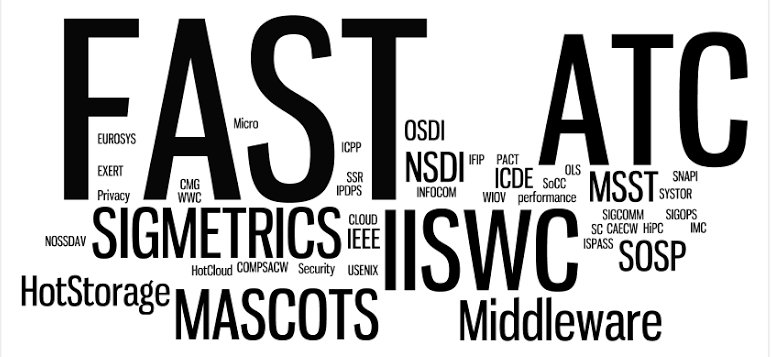
\includegraphics[scale=0.2]{presyn-figures/conference-names-wordle.jpg}} \hfill
    \subfloat[Year-of-publication tag cloud]{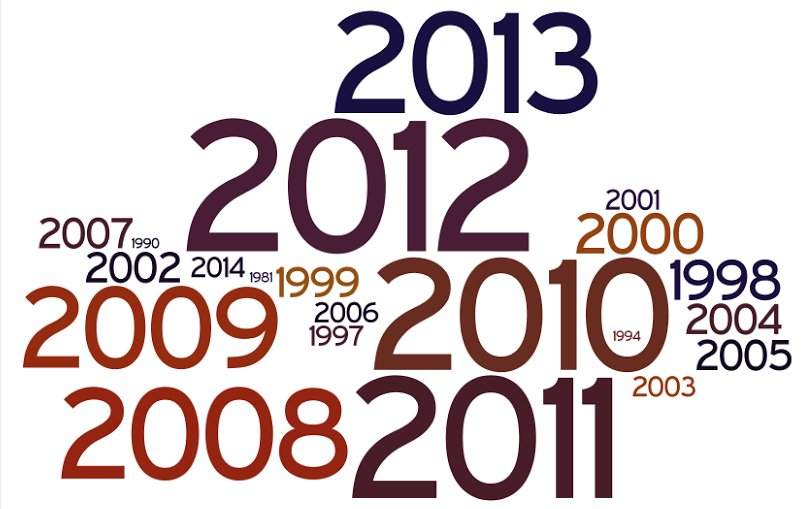
\includegraphics[scale=0.2]{presyn-figures/year-of-publication-wordle.jpg}}
    \\
    \caption{Representation of the conferences and the years of publication covered in our survey}
    \label{fig:tag-clouds}
\end{figure*}

%Due to above unsuccessful attempts at generating synthetic workload traces
%for evaluation of DRIVE, we once again turned towards datasets in literature
%and performed an extensive survey to determine whether any
%relevant useful datasets are available online.
We surveyed the datasets used in over
100 publications amounting to over 350 datasets\textemdash{}the tag clouds
in Fig.~\ref{fig:tag-clouds}(a) and (b) represent our survey coverage.
To begin with, we classified the dataset surveyed into
two sets: 
(i)~\textit{Proprietary datasets}\textemdash{}these are mentioned in various
papers but are not publicly available,
(ii)~\textit{Public datasets}\textemdash{}these are publicly available
online.
%and can be used by any researcher with an Internet connection.
%For example,
%the research groups from NetApp, IBM, etc use trace datasets that are
%internally available to them, but are not published online.
%For each of these datasets, we need to distinguish the dataset further based 
%on their context as follows:-
%(i)~Storage I/O traces with content representation,
%(ii)~Storage I/O traces without content representation,
%(iii)~Storage metadata with content representation, or
%(iv)~Storage metadata without content representation.
%The first item in the above list is the kind of trace we are looking for,
%i.e. I/O activity traces with content representation. However, we found
%that almost all of the public datasets available online fall in one of
%the other three categories listed above.

\paragraph{Proprietary datasets.}
Most datasets cited in literature are rarely hosted
publicly~\cite{generating-datasets}, hence unavailable to
other researchers for comparative analysis. 
We present a brief categorization.
%(In the thesis, 
%we cite the works which have used each category of dataset, although we
%omit that discussion here for the sake of brevity).

\begin{enumerate}
	\singlespacing
 \item \textit{Homes:} Shared-storage hosted home directories of
 employees or students or researchers.
 %~\cite{primary-data-dedup, backup-workloads-characterization, 
%datadomain, cifs-study, redundancy-alternatives}.
 \item \textit{CollaborationShares:} Shared-storage hosted directories
 among researchers or collaborators.
% created by one user and read/updated by many.
 %~\cite{content-sampling, idedup, cifs-study, redundancy-alternatives}.
 \item \textit{WebServer:} Webserver and Web-search workloads.
 %~\cite{storagecharacterization, filesystem-workloads, 
 %content-sampling, my-cache-or-yours, filesize-distrib-cause, 
 %web-cable-modem, scaling-phenomena, web-client-access-patterns}.
 \item \textit{SoftwareDeployment:} VM images, softwares, binaries 
	 for deployment by users.
 %~\cite{similarity, iodedup, redundancy-alternatives}.
 \item \textit{VM-Dataset:} VM images with
 different operating systems, applications and libraries.
 %~\cite{similarity, dedup-effectiveness}.
 \item \textit{VM-Backup:} VMs fully or partially backed up regularly, 
	 causing significant redundancies.
 \item \textit{DatabaseBackup:} Database backup storage and workloads.
 %~\cite{ddelta, hybrid-dedup, 
 %backup-workloads-characterization, ventana}.
 \end{enumerate}


\paragraph{Public dataset repositories.} 
%Below we provide a listing of those online trace repositories,
%which contain huge number of traces (i.e. multiple trace sets, not just one)
%and are available to the researchers for development and analysis of network
%and storage systems.
\begin{enumerate}
		\singlespacing
    \item \textbf{SNIA IOTTA Repository}: Provides storage-related I/O traces, tools and analysis.
    \item \textbf{HP Labs Repository}: Provides filesystem and application traces, albeit outdated.
    \item \textbf{UMass Trace Repository}: Provides network, storage, and other traces.
    \item \textbf{Internet Traffic Archive}: Provides access to traces of Internet network traffic.
    \item \textbf{VMware image repository}: Provides VMware images with various Linux distributions installed like CentOS, Debian, Fedora, FreeBSD and OpenSUSE.
    %\item FSL labs repository
    %\item LiveDFS repo?
\end{enumerate}

\paragraph{Public individual datasets.}
\begin{enumerate}
		\singlespacing
    \item \textbf{I/O deduplication traces}: Traces provided via~\cite{iodedup}, which we used in our evaluation.
    \item \textbf{Plan 9 traces}: Snapshots of Plan 9 filesystem deployed in Bell Labs research center. 
    \item \textbf{Animation-bear dataset}: NFS traces from animation company, released by HP Labs.
    \item \textbf{Linux kernel \& GCC sources}: Successive versions have overlapping content.
\end{enumerate}

Among the public repositories and the public individual datasets 
listed above, only the traces available via \cite{iodedup} 
are useful for our purposes.
All others are either storage metadata traces or I/O traces
without content representation, hence unfit for evaluation of I/O deduplication
techniques.

\paragraph{Public benchmarks.}
Some benchmarking tools and application benchmarks have also been used for
workload generation in literature. Some of the most popular benchmarks
for Storage I/O workload generation are: (i)~\texttt{Filebench}, 
(ii)~\texttt{dbench},
(iii)~\texttt{HiBench},
(iv)~\texttt{IOzone},
(v)~\texttt{IOMeter},
(vi)~\texttt{PostMark},
(vii)~\texttt{FIO},
(viii)~\texttt{CloudSuite},
(ix)~\texttt{TPC Benchmarks},
(x)~\texttt{SPEC Benchmarks},
(xi)~\texttt{NAS Parallel Benchmarks},
(xii)~\texttt{HPC Challenge Benchmark},
(xiii)~\texttt{PARSEC}.
%(xiv)~\texttt{Kernel compile benchmark}.

Most of the above benchmarks are either too simplistic or have so many
control knobs that it is a daunting task to choose the correct
settings~\cite{generating-datasets}.
Given any benchmarking tool which has several knobs that can be tweaked,
we might tweak the knobs exhaustively to determine those
settings which produce a compatible workload for I/O deduplication evaluation.
However, the onus of proving that the resulting tweaked workload is a
realistic workload would still loom large. We thus make the claim that,
after having established the initial worth of the DRIVE system using
the available traces, there is nothing more to be gained by evaluation
using synthetic benchmarks. Further evaluation of the DRIVE system is
valuable only if performed using real-world workloads or using ``realistic''
benchmarks.
\\
\\
%Based on our findings that (1) existing public datasets are not
%relevant for evaluation of I/O deduplication, (2) many relevant
%datasets are proprietary and not publicly-available, as well as,
%(3) existing benchmarks are not ``realistic'' enough for our purposes, 
%we turn to the next avenue of using real-world traces to build
%synthetic traces ourselves. We performed a detailed literature
%survey of this area (i.e., generating realistic traces) and
Our survey revealed that all efforts to generate realistic synthetic traces,
rely on characterization of some available real-world traces.
Therefore, next we perform trace characterization of the 
available \textit{homes} 
and \textit{webvm} traces,
which will be helpful to build realistic traces in future.

\subsection{Trace characterization of the available dataset}
In Table~\ref{tab:tracechar-summary-stats}, we present 
summary statistics regarding the traces\textemdash{}these are statistics reproduced
from the original paper~\cite{iodedup}.
We further characterize the traces by plotting distributions for 
the following four metrics, for both read and write requests:-
\begin{enumerate}
		\singlespacing
    \item Blocks accessed distribution: which block addresses receive most accesses?
    \item Run length distribution: how many consecutive blocks accessed?
    \item Reuse distance distribution: what is gap between successive access to a block?
    \item Jump length distribution: what is gap between blocks accessed in successive requests?
\end{enumerate}

 \begin{table}[t]
 \caption{Summary statistics of one week I/O workload traces \textit{webvm} and \textit{homes}~\cite{iodedup}}
%  \hspace{-0.2in}
 \begin{center}
 \begin{tabular}{|c|c|c|c|c|} \hline
   \bf{Workload} & \bf{Filesystem} & \bf{Memory} & \bf{Filesystem} & \bf{Filesystem size} \\
  \bf{type} & \bf{size (GB)} & \bf{size (GB)} & \bf{accessed (\%)} & \bf{(no. of 4KB blocks)} \\ \hline
  \textit{webvm} & 70 & 2 & 2.8 & 18 million \\
  \textit{homes} & 470 & 8 & 1.44 & 123 million \\ \hline
 \end{tabular}
 \label{tab:tracechar-summary-stats}
 \end{center}
 \end{table}

\subsubsection{Blocks accessed distribution}

%These figures were plotted directly from Octave, and hence having all
%this problem. The only thing good in Octave was that it could easily
%plot histogram with 25 bucket by hist(X, 25). Plotting has been a real
%pain though, so better to use [y, x] = hist(X,25) and then print out
%the x and y values, to use them separately in a gnuplot script with
%desired formatting.
%\hspace{-1in}
\begin{figure}[t]
    \centering
    \subfloat[Access distribution of blocks read (\textit{webvm})]{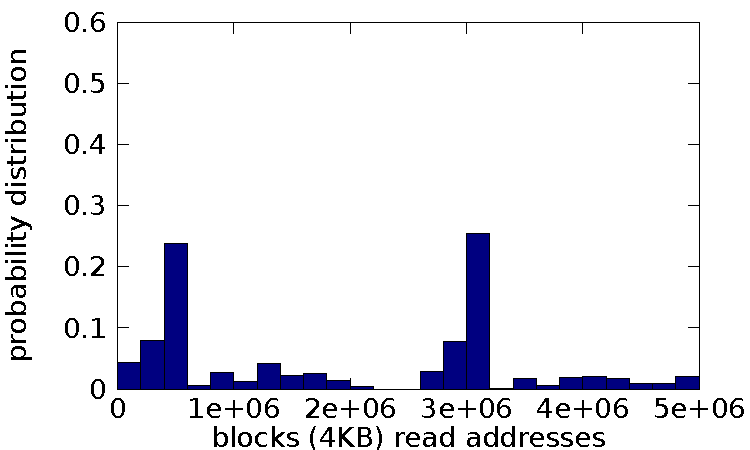
\includegraphics[scale=0.6]{tracechar-figures/21-day/webvm-block-read-appended-21-prob.pdf}}
    \hfill
    \subfloat[Access distribution of blocks written (\textit{webvm})]{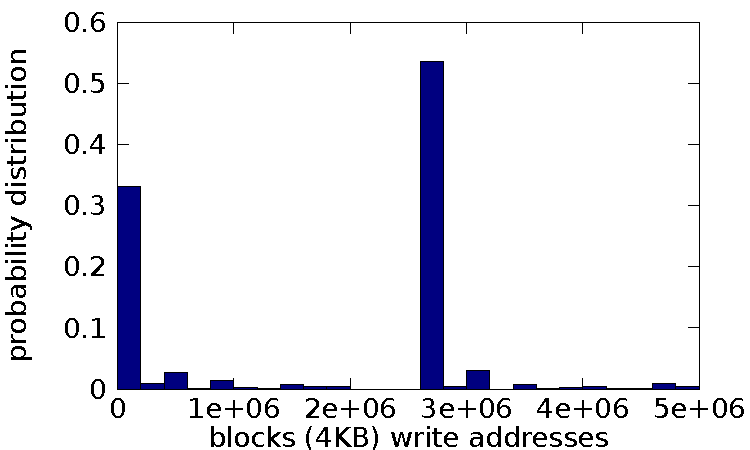
\includegraphics[scale=0.6]{tracechar-figures/21-day/webvm-block-write-appended-21-prob.pdf}}
    \\
    \subfloat[Access distribution of blocks read (\textit{homes})]{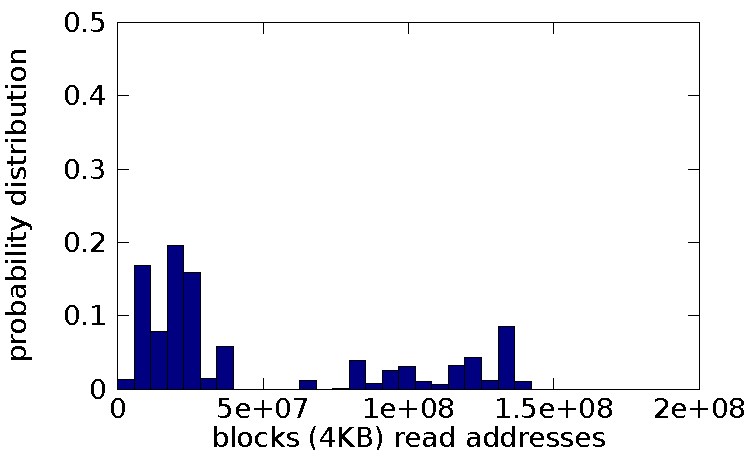
\includegraphics[scale=0.6]{tracechar-figures/21-day/homes-block-read-appended-21-prob.pdf}}
    \hfill
    \subfloat[Access distribution of blocks written (\textit{homes})]{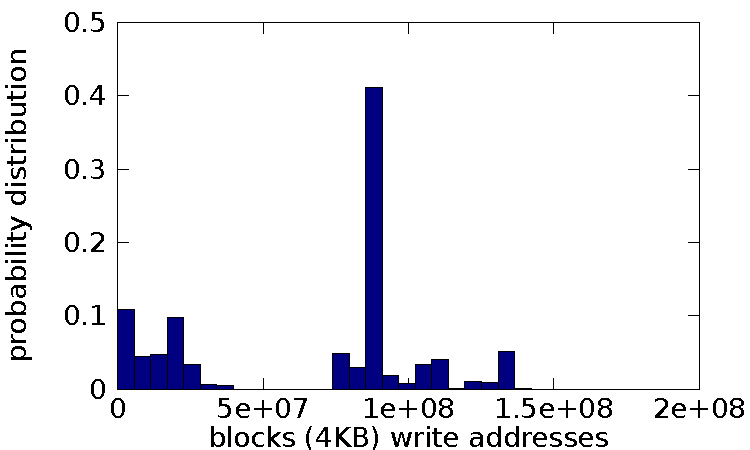
\includegraphics[scale=0.6]{tracechar-figures/21-day/homes-block-write-appended-21-prob.pdf}}
    \caption{Block access popularity distribution for reads and writes in
    \textit{webvm} and \textit{homes} traces}
    \label{fig:webvm-blocks-read-write-distrib}
\end{figure}

Fig.~\ref{fig:webvm-blocks-read-write-distrib}(a) presents a probability distribution
of the 4KB block addresses read in the \textit{webvm} trace,
while Fig.~\ref{fig:webvm-blocks-read-write-distrib}(c) presents the same
for the \textit{homes} trace. The x-axis plots the addresses of the blocks
read or written, respectively, such that each address is for a 4 KB block
or 8 sectors or 4096 bytes.
It can be seen that a major portion of
the read accesses in both traces are limited to only some portions of the address space,
while the rest of the address space gets much fewer read accesses.
Similar behaviour is observed in the write accesses as well, as shown
in Fig.~\ref{fig:webvm-blocks-read-write-distrib}(b)
and Fig.~\ref{fig:webvm-blocks-read-write-distrib}(d), respectively.
% Note that, though the
% x-axis limits are the same for both the read and write graphs, the y-axis ranges 
% are different\textemdash{}this is in line with the fact that the total number
% of reads in both the traces is lower than the number of writes.
Note that, the total range of blocks accessed is bigger in case of
the \textit{homes} trace as compared to the \textit{webvm} trace\textemdash{}this is
because the file system size in case of the former is around an order
larger than the latter, as shown in
Table~\ref{tab:tracechar-summary-stats}.

The above block accessed distributions prove that there is \textit{spatial locality} in
the blocks being accessed in the traces, i.e., the accesses tend to be clustered more
in particular regions instead of being uniformly distributed throughout the address
range. This behaviour is typical of most storage I/O workloads and several
models have been proposed in literature to capture this characteristic
into realistic benchmarks~\cite{jump-based-synthetic, storagecharacterization}.

\begin{figure}
    \centering
    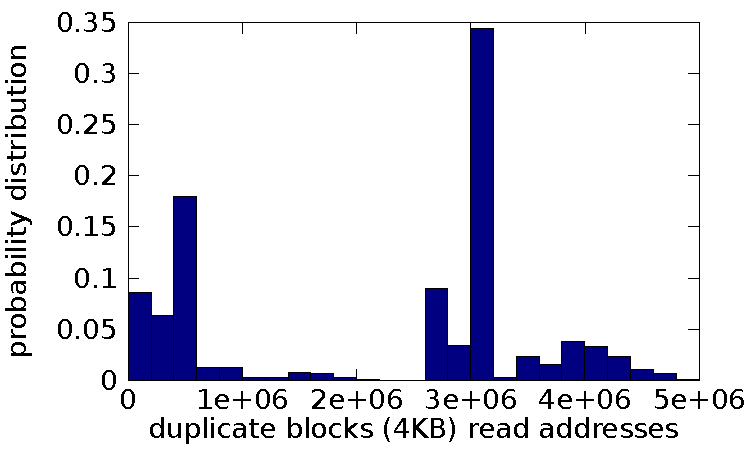
\includegraphics[scale=0.6]{tracechar-figures/21-day/webvm-dedup-block-read-appended-21-prob.pdf}
    \caption{Distribution of accesses of duplicate content blocks}
    \label{fig:webvm-blocks-dedup-distrib}
\end{figure}

Fig.~\ref{fig:webvm-blocks-read-write-distrib} refers to all (i.e., unique as well as
duplicate) blocks
being accessed in the trace, however since we are interested in I/O
deduplication, it would be interesting to know whether such spatial
locality of access exists for duplicate data as well. The work in
\cite{idedup} certainly demonstrates this to be true of real-world storage content,
however the question that faces us is whether this is true of I/O workloads
as well.
To answer this question, we
consider only those records from the trace which read ``duplicate''
data, i.e., each trace record considered in this scenario is associated
with content that has already been read or written in a previous trace
record. 
%For every block of content that we encounter in the trace, we
%assign it an index called the \texttt{dedupID} and if a content is
%repeated, it is assigned the same \texttt{dedupID} as the previous
%instance of that content in the trace. Thus, \texttt{dedupID} is a
%unique identifier for block content. and in
Fig.~\ref{fig:webvm-blocks-dedup-distrib}
plots the access distribution for only those content which were
found to be duplicate in the \textit{webvm} trace.
As expected, we can see in Fig.~\ref{fig:webvm-blocks-dedup-distrib}
that there is spatial locality within the accesses
of duplicate data as well.

\subsection{The need for I/O deduplication benchmarks}
%Further, we conclude that the next best way of
%preparing datasets for evaluation would be to synthetically generate
%realistic workload traces by capturing the characteristics of the
%available trace itself. Pursuant to this, we performed another detailed
%literature survey of relevant papers that develop a workload model
%based on measurements from real-world, and then
%generate synthetic realistic benchmarks using
%the developed model. The survey revealed that t
There is related work
that generates realistic benchmarks for I/O access (i.e. only concerned
with block numbers accessed, not their content) as well as for storage
deduplication (i.e. concerned with content stored on disk, not content
accessed). However, there is no related work so far that generates
realistic I/O access traces that account for the content as well.
In this section, we make the case that there is significant
literature in the areas of realistic benchmark generation for
network~\cite{echo} and
storage I/O performance~\cite{storagecharacterization} as well as 
storage deduplication
evaluation~\cite{generating-datasets}, but none in the area of I/O deduplication.

\subsubsection{Generating realistic storage I/O performance benchmarks}
The generation of realistic I/O performance benchmarks
has received considerable attention in recent literature~\cite{storagecharacterization,
jump-based-synthetic, distiller}.
The work in~\cite{storagecharacterization}
builds a Markov model to capture \textit{spatial locality},
with each state representing one-quarter of the
block address range (called logical block number range or LBN range)
and each transition representing
the probability of transitioning from one LBN range to another. The idea
is that due to the spatial nature of the workload, most of the
transitions would stay within the same state and the probabilities
of transitioning out of one state to another would be quite low.
%Thus, a request stream is perceived as a state machine
%which transitions between LBN ranges with certain probabilities.

The work in \cite{jump-based-synthetic} claims that to characterize
and recreate a realistic storage I/O workload, it is necessary to not
only capture the block accessed distribution, but also the jump distance
distribution. The approach proposed is to transform the synthetic 
trace generation problem into the
Hamiltonian Path problem, and then to apply a brute-force, depth-first
search to find a Hamiltonian path (this path is expected to have the
same jump distance characteristics as the original trace).
The work in \cite{distiller} acknowledges the challenge that synthetic
workloads are accurate only if they share certain key properties
with the original production workload(s). 
%The unfortunate aspect
%is that it is not known which properties are ``key'' for
%any given workload or storage system. Thus, regarding the selection
%of key properties for workload characterization
%and generation, the work in \cite{distiller} presents 
A tool called \texttt{Distiller} is presented, which automatically picks
them from a library of attributes, using an iterative trial-and-error method. 
%As input, the
%\texttt{Distiller} tool needs a library of workload attributes,
%from which it picks one additional attribute at each iteration,
%and checks whether the chosen set of attributes is representative
%enough of the given workload. If so, the modeling is done and
%if not, it chooses one more attribute in the next iteration
%and so on until a realistic representation is achieved.

%\subsubsection{Realistic network activity modeling and benchmark generation}
%The work in \cite{echo} presents a modeling scheme called ECHO, which
%captures the temporal and spatial behaviour of network traffic in
%large-scale datacenter applications. Two models are built, wherein
%the first is a distribution-fitting model (called the \textit{single-server temporal
%model}) that generates per-server
%network traffic and the second is a Markov chain model (called the \textit{system-wide
%spatial model}) that captures
%server-to-server interactions.
%
%\begin{figure}[t]
%    \centering
%    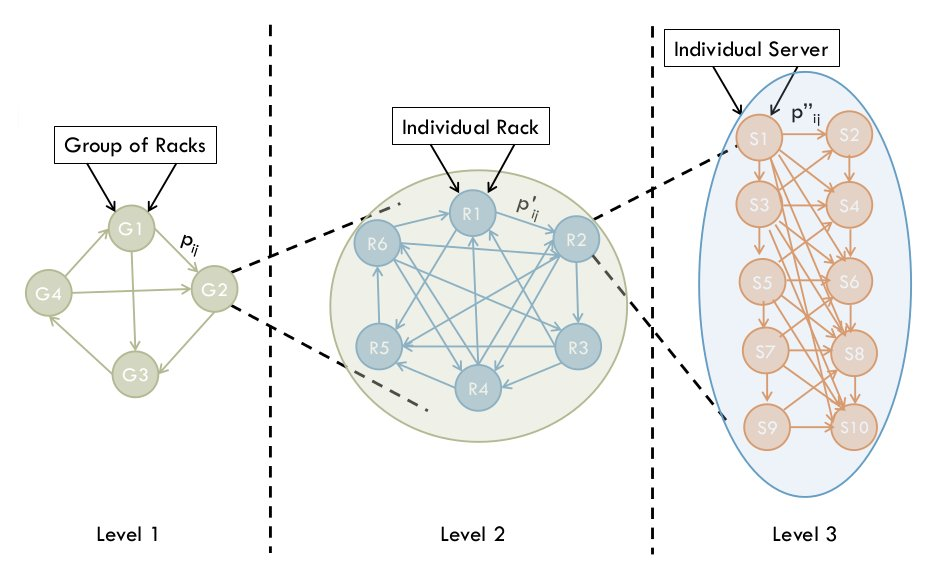
\includegraphics[scale=0.4]{presyn-figures/echo.jpg}
%    \caption{Schematic of the hierarchical spatial Markov chain model~\cite{echo}}
%    \label{fig:echo}
%\end{figure}

\subsubsection{Generating realistic file system benchmarks}
The work in \cite{impressions} is motivated by
the key properties to realistically represent a filesystem
image. Depending on the workload to
be emulated, the filesystem image may
need different levels of detail. For example, a data mirroring
scheme like RAID or a system that takes full backups would be
independent of both metadata and content.
On the other extreme, a search engine's performance
would depend on both the metadata and the exact content
on which it operates.

\subsubsection{Generating realistic storage deduplication benchmarks}
To justify creation of benchmarks for storage deduplication, the work in
\cite{generating-datasets} claims that the benchmark or datasets should be:-
\begin{enumerate}
		\singlespacing
    \item Sufficiently large
    \item Having controllable characteristics
    \item Easy to distribute to other researchers
    \item Easily accessible or reproducible by other researchers
    \item Realistic
\end{enumerate}
Due to above conflicting requirements, the work in \cite{generating-datasets}
presents a framework which captures the important characteristics
of a real-world workload into a model with a relatively
smaller footprint, for easy distribution. 
Benchmarks are generated which capture the changes in filesystem 
across multiple snapshots along-with its content
representation, using a combination of a
Markov model and a multi-dimensional distribution model.
\\
\\
Based on the above surveyed literature, we conclude that there are no
realistic benchmarking tools or trace generation frameworks 
for evaluation of I/O deduplication techniques. Thus, 
researchers need to either collect multiple
production workload traces for their own research, or create frameworks
that can synthesize realistic I/O traces along-with content representation.

